\documentclass[aasms,12pt]{article}
\usepackage{natbib}
\setlength{\bibsep}{0pt plus 0.3ex}
\usepackage[margin=1in]{geometry}
\usepackage{sectsty}
\usepackage{graphicx}
\usepackage{hyperref}
\usepackage{epstopdf}
\usepackage[skip=2pt,font=small]{caption}
\captionsetup{width=\textwidth}
\usepackage{amssymb, amsmath, amsfonts, xcolor}
\hypersetup{
    colorlinks,
    linkcolor={red!50!black},
    citecolor={blue!80!black},
    urlcolor={blue!80!black}
}


\sectionfont{\normalsize}
\subsectionfont{\small}


%\citestyle{aa}
\newcommand{\apj}{The Astrophysical Journal}
\newcommand{\apjl}{The Astrophysical Journal Letters}
\newcommand{\apjs}{The Astrophysical Journal Supplemental Series}
\newcommand{\aap}{Astronomy \& Astrophysics}
\newcommand{\aaps}{Astronomy \& Astrophysics Supplemental Series}
\newcommand{\mnras}{Monthly Notices of the Royal Astronomical Society}
\newcommand{\baas}{Bulletin of the American Astronomical Society}
\newcommand{\zap}{Zeitschrift für Astrophysik}
\newcommand{\sol}{\ensuremath{\odot}}
\newcommand{\RB}{Rayleigh-B\'{e}nard }
\newcommand{\grad}{\ensuremath{\nabla}}

\usepackage{fancyhdr}
\pagestyle{fancy}
\fancyhf{} % sets both header and footer to nothing
\renewcommand{\headrulewidth}{0pt}
\cfoot{\footnotesize{\thepage}}





\begin{document}
\begin{center}
   \large\textbf{Constraining magnetic and angular momentum transport in stellar envelope convection from the smallest to largest scales}\\
   \vspace{0.2cm}
   \large{Evan H. Anders}\\
   \vspace{0.2cm}
\end{center}

\vspace{-0.6cm}

\section{The need for improved modeling of rotation on solar and stellar magnetism}

\subsection{Understanding stellar structure in the asteroseismic age}
The advent of asteroseismic science has closely paralleled that of exoplanetary science.
The early small samples of stellar pulsations obtained by ground-based observatories \citep[e.g.,][and others]{kjeldsen&frandsen1991, bouchy&carrier2001, bedding&all2001} have given way to datasets of more than $10^4$ stars \citep[e.g.,][]{yu&all2018, santos&all2019b} in the age of CoRoT, Kepler, and K2 data.
With another 20,000 asteroseismically-interesting targets in the TESS satellite's two-year nominal mission \citep{schofield&all2019} and more interesting data from the future WFIRST and PLATO missions, it is expected that by 2030 we should have observations of $10^7$ pulsating red giants and $10^5$ dwarfs and subgiants in hand  \citep{huber&all2019}.
In addition to learning about the nature of stars aside from our Sun, asteroseismology enables us to fairly accurately determine the age of stars, thus enabling galactic archaeology, in addition to enabling us to determine the mass and radius of stars with solar-like pulsations, thus enabling the measurement of exoplanetary radii from the transit method.
Asteroseismic measurements generally rely on stellar structure models, and these models have some known deficiencies \citep{buldgen2019}, in particular their handling of complex phenomena like rotation, convection, and magnetism.
With the exponential rise in asteroseismic targets, and the projected continuation of this rise, it is crucial that the we continue to invest in the theory informing these stellar models and measurements.

The state-of-the-art method for obtaining stellar strucuture data is the use of one-dimensional models of stellar interiors from codes like MESA \citep{paxton&all2011}.
The coupling of MESA models and the GYRE code \citep{townsend&teitler2013} has enabled efficient identification of pulsational modes in a wide variety of stars.
Unfortunately, MESA models necessarily depend on one-dimensional parameterizations of convection and often employ the decades-old mixing length theory \citep[MLT,][]{bohm-vitense1958}.
MLT does an adequate job of describing convection within stars, but there are some well-known instances in which it regularly fails.
For example, 1D stellar models do not correctly produce the surface layers of stars with convective envelopes, but recent work suggests they fare better when coupled with three-dimensional surface simulations \citep{jorgensen&weiss2019}.
Furthermore, these one-dimensional models assume spherical symmetry and generally neglect the effects of rotation and magnetism.
The numerous observations of flare stars and recent asteroseismic observations which have detected magnetic field-induced frequency shifts \citep{santos&all2018} suggest that magnetism should not be neglected, and recent work shows that the specific configuration of the magnetic field impacts asteroseismic measurements \citep{thomas&all2019}.
Furthermore, it is well known that the sun exhibits differential rotation characterized by latitudinal variations in its rotational profile in the solar convection zone \citep{thompson&all1996, schou&all1998}, and differential rotation has now been observed in stars beyond the Sun \citep{benomar&all2018}.
These observations all suggest that a 1-dimensional parameterization of convection, and a neglection of complicating effects, cannot sufficiently capture the complexities of stars.

\subsection{The Solar Convective Conundrum}
The Sun is our closest star, and the only star for which we have high-resolution, spatially-resolved observations in years-long datasets.
These datasets have enabled helioseismic measurements of the solar interior, resulting in our modern understanding of the solar differential \citep{schou&all1998} among other complex flow structures such as meridional circulation.
In addition to revealing large-scale internal structures in the Sun, the observational constraints being placed by helioseismology have called into question our fundamental understanding of the nature of solar convection.
Observations by \citet{hanasoge&all2012} place an upper limit on convective velocity magnitudes nearly two orders of magnitude lower than those predicted by simulations or MLT.
Other heliseismic measurements using different techniques claim detections of velocity magnitudes more in line with what is expected from theory \citep{greer&all2015}, but observe an unexpected decrease in powers at large scales compared to simulations.
Even observations of convective motions at the solar surface \citep{hathaway&all2015} do not observe these anticipated, large-scale ``giant cells.''
These observations constitute a piece of the Solar Convective Conundrum, and much theoretical work over the past decade has aimed to grasp what piece, or pieces, of physics long-standing models like MLT are missing.
Two primary hypothesis aiming to explain the lack of giant cells in the Sun are the ``Entropy Rain'' hypothesis and a suggestion that the solar convective interior is rotationally constrained.

The entropy rain hypothesis, first suggested by \citet{spruit1997}, suggests that downflows alone carry the solar luminosity through the solar convection zone, and has been preliminarily incorporated into a modified mixing length theory by \citet{brandenburg2016}.
Some simple simulations of \citet{kapyla&all2017} suggest that indeeed downflows may be more important than upflows in determining convective properties in stellar envelope convection.
Recently, I conducted high resolution simulations of one possible dynamical manifestation of entropy rain: atmospheric thermals in stratified domains \citep{andersLB2019}.
We found that such a mechanism could plausibly carry the solar luminosity in the deep solar convection zone through their enthalpy fluxes.
However, even if such a mechanism could carry the solar luminosity, the manner in which these entropy rain droplets transport angular momentum and magnetic fields is deposited could have huge implications for flow structures within the Sun.

It has also been suggested that the effects of rotation alone may be sufficient to explain the solar convective conundrum \citep{featherstone&hindman2016}.
These simulations show that as the degree of rotational constraint, characterized by the Rossby number, increases, so too does the spherical harmonic degree of maximum velocity power of the convection.
However, simulations of increasingly rotationally constrained convection typically show \emph{anti-solar} differential rotation, rather than solar-like.
Global simulations which both suppress giant cells and correctly produce the solar differential rotation profile have not been achieved.

Over the course of my postdoctoral studies, I will examine the importance of rotation on stellar convection and stellar structure from the smallest to the largest scales.
The small scale (thermal, or plume) experiments, described below in section \ref{sct:thermals}, will aim to continue to verify whether or not entropy rain is a feasible mechanism for transporting stellar luminosity in lower main sequence, solar-like stars.
The largest scale (global spherical simulations) experiments, described below in section \ref{sct:global_models} will simultaneously develop community tools to use in studying rotating convection, and also apply those tools to simulate increasingly rotationally constrained, turbulent simulations.
I will use the Dedalus pseudospectral framework \citep{burns&all2019}, which I have become proficient at using during my graduate career, to carry out these investigations.


\section{Vector transport by convection at the smallest scales}
\label{sct:thermals}
Stellar convection is a turbulent process.
While modern computers are incapable of simulating small-scale fluid motions at Reynolds and Peclet numbers like those present in the Sun, modern simulations can achieve turbulent dynamics (see e.g.,).
I propose to gain insight into the mechanisms that stellar convection utilizes to transport vector fields by studying dynamics of convection at the smallest scales in order to understand turbulent effects.
Furthermore, most simulations of compressible convection to date are in the high Mach number limit; however, through clever use of numerical techniques we are now capable of studying low Mach number, fully compressible convection \citep{anders&brown2017}.
Much of the convection in the envelopes of lower main sequence stars is thought to be at Mach numbers much lower than unity, and so a detailed understanding of the manner in which convective transport differs in this regime compared to the high Mach number regime is crucial.

In order to determine the nature of vector transport by turbulent, low Mach number convection, I will use two styles of simulations as laid out below in task A and task B.

\subsection{Task A: Vector transport by individual thermals}
Thermals are regions of cold (or hot) fluid which accelerate due to buoyancy forces.
During a spin-up period, thermals shape themselves into buoyant vortex rings, and the vorticity of these rings entrains environmental fluid, causing these structures to grow \citep{lecoanet&jeevanjee2019}.
Thermals are well understood in the Boussinesq limit and have been studied extensively in the atmospheric context, and are thought to be the nucleus of the cloud formation process in Earth's atmosphere.
Recently, I studied thermals as a model for solar convection and came to understand the effects of stratification on the propagation and entrainment properties of thermals \citep{andersLB2019}.
I conducted high resolution simulations of these thermals, showed that their evolution agreed well with our developed theory, and demonstrated that if solar downflows behave like thermals, as in the entropy rain hypothesis, the solar luminosity could feasibly be carried by downflows alone in the deep solar interior.
One benefit of studying thermals is that they are discrete fluid events that are simple to simulate from initial conditions until they reach their final state.
\emph{Plumes}, or continuously cooled regions of fluid, are likely a better model for surface downflow lanes in solar surface convection.
However, past work has shown that in stratified domains, buoyant vortex rings pinch off of plumes and continue to propagate downwards.
As a result, the vortex ring evolution of thermals is perhaps an excellent model for solar downflows at the smallest scales.
As past results (Glatzmaier) have shown that downflows in convection can effectively pump magnetic fields downwards and current results \citep{kapyla&all2017} suggest that downflows are likely more important than we recently thought, thermals provide an excellent tool for understanding how important small scale motions are for vector transport.

In \citep{andersLB2019}, we studied thermals in the laminar regime.
The thermal simulations in \citet{andersLB2019} had a characteristic Reynolds number of approximately 600 \emph{on the length scale of the thermal}.
Such a Reynolds number is difficult if not impossible to achieve on the length scale of downflow lanes in global simulations of convection.
During my postdoctoral studies, I will extend my study of stratified thermals to those which are truly turbulent, whose Reynolds numbers are 6000.
This has already been achieved in the Boussinesq limit by \citet{lecoanet&jeevanjee2019}, and initial results show that resolving the dynamics of thermals at these values in stratified domains is possible.

In \citet{andersLB2019}, we came to understand the scalar transport properties of these thermals with depth in nonrotating, nonmagnetized domains.
While the thermal simulations I studied previously had two fundamental control parameters (the degree of dissipation or turbulence, characterized by the Reynolds number, and the degree of stratification).
I now propose incorporating rotational and magnetohydrodynamical effects into these simulations.
All simulations will be decomposed in Dedalus using a (vertical) Chebyshev basis and two (horizontal) fourier bases.
Laminar simulations will simulate up to a coefficient resolution of 512x256$^2$, and each simulation in this regime represents roughly 25,000 cpu-hours.
Turbulent simulations will simulate up to a coefficient resolution of 1024x512$^2$, and each simulation in this regime represents approximately a quarter of a million cpu-hours.

\subsubsection{Task A.1: Transport of angular momentum by thermals}

\begin{figure*}[t!]
    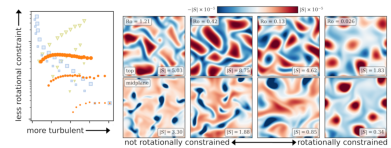
\includegraphics[width=\textwidth]{./figs/rossby_plot.png}
    \caption{ 
	\label{fig:rossby_plot} }
\end{figure*}

During my doctoral work, I studied rapidly rotating convection in f-plane cartesian atmospheres \citep{anders&all2019}, and I propose to study thermals in similar domains.
Placing thermals in f-plane atmospheres adds two additional axes to the parameter space of the problem: latitude, and importance of rotation (characterized by a Rossby number)
I will first study an initial suite of simulations in the laminar regime in order to verify how the manner in which entropy rain deposits angular momentum as a function of both stellar latitude and the Rossby number.
After characterizing the behavioral regimes of thermals as a function of latitude and rotational constraint, I will target each of these behavioral regimes with smaller suites (3-5 simulations) in the turbulent regime.
These simulations will allow us to determine whether or not solar downflows could reasonably establish the solar meridional circulation or differential rotation profiles.
Furthermore, we will find whether certain degrees of rotational constraint or latitudes prevent downflows from transiting convective envelopes.

\subsubsection{Task A.2: Transport of magnetic fields by thermals}
The second suite of proposed simulations is in plane-parallel boxes in nonrotating reference frames.
The inclusion of magnetism again adds two new parameters: the magnetic prandtl number, indicating whether or not magnetic fields are highly diffusive, and a measure of the strenght of the magnetic fields, similar to a plasma beta or the Chandrasekhar number in magnetoconvection.
In addition to these new parameters, the inclusion of magnetism requires a choice of initial magnetic field setup.
Two obvious choices are one in which the thermal is launched in a strong background magnetic field, and one in which the magnetic field is localized in a thin horizontal sheet (Glatzmaier).

\subsection{Task B: Vector transport by time-evolving convection in plane-parallel atmospheres}
While the thermal simulations conducted in Task A will allow for detailed study of the manner in which individual dynamical events transport these vector fields of interest, direct measurements of the effects of an ensemble of convective elements are impossible in those simulations.
The next phase of my postdoctoral studies will take one step to larger length scales, and rather than studying individual downflows will study an ensemble of downflows in a local, plane-parallel box.
Such local simulations have been used to great effect in the solar community due to their less expensive nature than global simulations.

Here, these simulations will contain a simple model of the convective region of a solar like star: an upper region which is unstable to convection connected to a lower region which is convectively stable.
The basic parameters of such a setup are the degree of stratification, the Mach number of the convection, and the stiffness of the stable region (or, how effectively convective motions are able to continue propagating into that stable region).

I don't know what the main question is that's going to be studied in the rotating regime.

It's often thought that downflows pump magnetic field down into the tachocline, but is that possible if you have a stiff interface between the stable and convective region?
In this case, does the magnetic field stay available for the convection?

\section{Accelerated Vector Transport in Global Simulations}
\label{sct:global_models}
\subsection{Building the tools for accelerated global simulations}
The experiments laid out in section \ref{sct:thermals} will be foundational for the capstone projects of my postdoctoral studies: global simulations of rotating convection and magnetoconvection in spherical domains.
Studies of global dynamo simulations have provided fascinating insight into the workings of stellar convection, including showing us that stars can self-consistently generate wreaths of magnetism and undergo magnetic polarity changes such as those observed in the solar dynamo.
Global simulations have also presented a perplexing result in relation to the Sun's differential rotation profile.
The Sun has a fast-rotating equator (rotates every 25 days) and slow rotating poles (rotates every 35 days), and deep convection is believed to be rotationally constrained.
However, when global simulations examine rotationally constrained convection, they find \emph{antisolar} differential rotation (fast poles, slow equator).
The belief that deep convection is rotationally constrained is, however, fairly well-founded in mixing length theory, and recently it has been suggested that a rotationally constrained interior may be a solution to the suppression of giant cells in the Sun \citep{featherstone&hindman2016}.
These two results are counter to one another: the Sun may need to be rotationally constrained given the flows that we see at the surface, but if it is rotationally constrained, then how did it establish its differential rotation profile?

Unfortunately, global simulations are costly.
The wall time of state-of-the-art, marginally turbulent simulations which display interesting dynamo or rotational statistics are often quoted on timescales of months to roughly a year.
Some of these costs are unavoidable: highly resolved turbulent simulations necessarily take small timesteps, and therefore results come slowly.
However, some of the expense of these simulations is in some cases time wasted.
System structure and mean flows, such as differential rotation, often build up on the order of \emph{diffusive} timescales, rather than convective overturn timescales.
As we strive to push simulations into increasingly realistic regimes, the separation between these timescales becomes more extreme, and it can take thousands of overturn times for one diffusive time to pass.
These long evolutionary timescales are a problem, because they limit our ability to understand the dynamical nature of convection in the Sun.

During my graduate career, I studied a mechanism for accelerating the long thermal relaxation timescale in convective systems.
This mechanism is published for Boussinesq convection \citep{anders&all2018} and has been adapated to stratified, compressible convection in plane-parallel systems within our research group to be used in forthcoming work.
At even modest values of the Rayleigh number, we found that we could reach a converged state using an order of magnitude fewer computational resources than when waiting for a standard thermal relaxation timescale.
These speedups make achieving thermal relaxation in moderately turbulent systems much less computationally expensive and also allow us to study converged dynamics in more turbulent, stellar-like simulations than would otherwise be achievable on modern computing resources.

During my postdoctoral studies, I propose extending my accelerated evolution (AE) method to the transport of vector properties in global simulations.
This extension will be grounded in the theoretical understanding gained at the small scales discussed in section \ref{sct:global_models}.
In essence, the procedure described in \citet{ander&all2018} is one which allows the user to take timesteps for the mean state and the mean flows which are much larger than those allowed by convection.
As I did in \citet{anders&all2018}, I will verify that this method produces the same results as a long relaxation in modest parameter regimes to build trust in the method.
Once this trust is established, this tool can feasibly be employed in extreme parameter regimes that are interesting and otherwise unfeasible to explore.
Once developed, this tool will of course be made publicly available.

After developing this tool, I will use it to try to determine if global simulations can be produced which both suppress giant cells and properly create the solar differential rotation profile.
The overturn timescale predicted by MLT for deep convection and the solar rotational timescale are both approximately one month, and so it is possible that the Sun is in an interesting transitional regime between nonrotating and rotationally constrained convection.
I will use the tools I develop here to densely sample parameter space in this regime in order to verify whether or not solar-like convection can be observed.
In my graduate studies I determined that the degree of rotational constraint in convective simulations in cartesian domains can be straightforwardly specified \citep{anders&all2019}, so this should be quite achievable.

I need to add something here about magnetic fields.

\subsection{Linking 3D tools to stellar structure evolution}

In addition to helping solve the convective conundrum, these accelerated evolution tools could have great benefits for asteroseismic research.
New research is beginning to couple three-dimensional, global simulations with 1-dimensional stellar structure tools in order to more accurately produce stellar structure profiles \citep{jorgensen&weiss2019}.
The fast equilibration of angular momentum and thermal profiles described here is essentially equivalent to taking timesteps which superstep the convective motions, similar to those taken in any one-dimensional stellar structure model.
These techniques presented here would therefore allow the coupling of 1-dimensional stellar structure codes with realistic statistics from three-dimensional convection to create converged stellar profiles.
Since stellar rotation times are relatively easy to measure from lightcurve data, asteroseismic inversions could take advantage of stellar structure profiles specifically evolved using three-dimensional convection and the proper degree of rotational constraint once these tools are developed.

\section{Collaborative studies at CIERA and Northwestern University}
\label{sct:northwestern}
\begin{itemize}
\item Daniel \& Yoram
\item Cross-disciplinary awesomeness of CIERA %(https://ciera.northwestern.edu/directory/?filter_keyword=&filter_tax_ciera_person_type=all&filter_tax_ciera_research_topic=all&filter_tax_ciera_research_method=theory-computational)
\item Arriving when CIERA is moving to its new building -- fresh start.
\item HPC: (https://ciera.northwestern.edu/high-performance-computing/). Two clusters. CIERA cluster (9 nodes x 28 cores). Northwestern Quest supercomputer 11,800 cores.
\end{itemize}


\section{Teaching and Outreach}
\label{sct:outreach}
The path to a career in the US STEM workforce is a leaky pipeline.
Data show that in particular, underrepresented minority groups and women pursue careers in STEM fields at a rate which is disproportionately low compared to the share of the total population that those groups constitute \citep{corbett&hill2015, nsf2019}.
While a great deal of focus is rightly placed on changing the career outlooks of these groups before the collegiate level, the pipeline continues to leak at the baccalaureate and post-baccalaureate levels, and underrepresentation becomes more severe.

During my graduate studies, I spent three years working with the University of Colorado's CU-STARs group.
CU-STARs is a combined ``outreach'' and ``inreach'' program with the dual aims of increasing STEM engagement for students at underserved, rural schools across Colorado while decreasing attrition of underrepresented groups in CU Boulder's Astrophysical and Planetary Sciences department.
Undergraduate students from CU in this group, or ``STARs,'' are provided with an inclusive community, peer mentoring (graduate student - undergraduate pairs), and opportunities to develop scientist skills.
In turn, STARs are also given opportunities to teach high schoolers about fun topics in astronomy and astrophysics with hands-on demos.
My role as a graduate student administrator in this group was to help coordinate, plan, and run outreach trips to rural schools across Colorado, mentor undergraduate students, develop courses and demo materials for courses in exoplanety discovery via the transit method, black holes, and atmospheric fluid dynamics.



\subsection{Outreach: Reach for the stars}
Reach for the Stars does a great job of engaging high school students with STEM in an authentic, inquiry-based way.
Discussion of why authentic experiences in scientific inquiry are important.
Discussion of the cool stuff that Reach for the Stars is already doing.
Name-drop of NSF funding.

Here's what I'd like to bring to the program:
\begin{itemize}
\item Professional development of graduate student fellows through in-depth redesign of inquiry activities and backwards design process.
\begin{itemize}
\item backwards design
\item assessment and teaching as a scientific discipline
\end{itemize}
\item 
\end{itemize}


\subsection{Inreach: Peer mentorship for the retention of undergraduates and early graduate students}
Mentoring has long been known to play a significant role in increasing retention and helping new departmental members acclimate to the department climate \citep{hunt&michael1983}.
Establishing robust mentoring programs based on evidence and knowledge of the recent literature in mentorship \citep[as in e.g.,][]{crisp&all2009, crisp&all2017} can be one critical component of helping broaden participation of underrepresented and marginalized groups in the STEM workforce.
During my years at Northwestern, I propose to work with the experts in Northwestern's \href{https://www.northwestern.edu/searle/index.html}{Searle Center for Advanced Teaching and Learning} to develop peer mentoring programs within Northwestern University's applied math department and the department of physics and astrophysics.
The goal of this program will be to connect entering undergraduate or graduate students mentees with mentors who are a few years more developed in their career.

Things that I need to think about more:
\begin{itemize}
\item mentor training
\item coffee funds
\item schedule and frequency
\item post docs?
\end{itemize}



\subsection{My career development}



\section{Summary and Perspectives}
\label{sct:summary}

\bibliographystyle{apj}
\bibliography{biblio}
\end{document}
